\documentclass[a4paper,titlepage]{article}
\usepackage[utf8]{inputenc}
\usepackage{fullpage}
\usepackage{indentfirst}
\usepackage[per-mode=symbol]{siunitx}
\usepackage{listings}
\usepackage{graphicx}
\usepackage{color}
\usepackage{amsmath}
\usepackage{array}
\usepackage[hidelinks]{hyperref}
\usepackage[format=plain,font=it]{caption}
\usepackage{subcaption}
\usepackage{standalone}
\usepackage[nottoc]{tocbibind}
\usepackage[noabbrev,capitalize,nameinlink]{cleveref}
\usepackage{titlesec}
\usepackage{booktabs}
\usepackage{csvsimple}
\usepackage[super]{nth}

% Custom commands
\newcommand\numberthis{\addtocounter{equation}{1}\tag{\theequation}}
\newcommand{\code}[1]{\texttt{#1}}
\newcolumntype{P}[1]{>{\centering\arraybackslash}p{#1}}

\titleformat*{\section}{\normalsize\bfseries}

%opening
\title{
	\textbf{ECSE 526 \\ Assignment 3}
	\\ \large Reinforcement Learning
}
\author{Sean Stappas \\ 260639512}
\date{November \nth{7}, 2017}

\begin{document}
	\sloppy
	\maketitle
	\twocolumn
	
	\section*{Introduction}
	
	
	\section{Description of approach to generalization}
	% 10. provides expression for distance metric between two states and describes state representation used by the RL agent, also includes rationale for choice of components of the distance metric
	
	Q-learning is the learning algorithm chosen for the agent. Many different distance metrics were used in the program, and close states are grouped based on this distance, as described by Mahadevan and Connell \cite{mahadevan}. Here are three simple distance metrics, with the rationale for each choice of components.
	
	\begin{description}
		\item[Manhattan] The \textsc{Manhattan} distance represents how close two states are on the Qbert pyramid, i.e., the number of blocks between them. This is a natural representation of distance in this environment, since Qbert can only change state by switching blocks and can only travel one block at a time (with the exception of using disks to jump back to the starting position).
		
		\item[Hamming] The \textsc{Hamming} distance represents the number of different state bits between two given states. The rationale behind this distance metric is that nearby states should have a similar bit pattern, assuming a sane state representation.
		
		\item[SameResult] The \textsc{SameResult} approach groups adjacent states together, such that, whenever a Q-update occurs for a certain Qbert position, all possible states that could have directly led to that state also get updated. The rationale here is that, for most states in the Qbert world, the path Qbert takes to get to that state is usually not important.
	\end{description}
	
	Many different state representations were used with varying results. First, a state representation was used keeping track of the color of every block, the position of disks, Qbert's position, the position of enemies (purple agents) and the position of friendlies (green agents). While this state representation completely encapsulates Qbert's world, it is very verbose and intractable if not using any distance metric, as described previously.
	
	With 21 blocks in the pyramid, an agent has 21 possible positions, representing 5 bits of entropy. This applies for Qbert, the enemies and the friendlies. A simple representation of the colors of the blocks can indicate if the block color is the goal color or not. With this binary value for each block, the colors can be represented with 21 bits. Finally, there are 12 possible locations for the disks, with each disk either being present or not, representing 12 bits of entropy. With all these elements in a state representation, we would need a total of $5*3 + 21 + 12 = 48$ bits to represent a state completely. This represents a state space with $2^{48} \approx 3 \times 10^{14}$ states. Clearly, this number of states is intractable for learning, showing the necessity for generalization with an appropriate distance metric. This state representation is called \textsc{Verbose}.
	
	Another approach to generalization is to use a simpler state representation. A simpler state may not completely represent the game world, but can be enough for an agent to learn how to behave correctly. For example, instead of keeping track of all enemies and all blocks, one can only keep track of enemies and blocks around Qbert, since that is what is important for Qbert. One problem with this approach, however, is that it can be hard for the agent to learn to go towards all the blocks in a level to change all the colors and finish the level. More information, such as the number of colored blocks on the board, can then be provided as well. This state representation is called \textsc{Simple}.
	
	Finally, another way to deal with a very large state space is to separate the learning problem into sub-tasks, allowing components of the state to add in complexity instead of multiply. Indeed, if we have separate tasks of enemy avoidance, friendly catching and block finding, we can have a simple specialized state for each task. This is the \textsc{Subsumption} model described by Mahadevan and Connell \cite{mahadevan}, and is explored further in \cref{sec:performance}.
	
	\section{Results of generalization}
	% 10. results provided for at least 3 different generalization approaches (i.e., choice of components of the distance metric) and meaningful discussion regarding consequences to behaviour of game agent
	
	The results of using the previous three distance metrics can be seen in...
	
	\section{Description of approach to exploration}
	% 10 provides expression for optimistic prior for (state, action) pairs with clear explanation of how agent chose action at each step and convincing rationale for the approach taken
	
	First, the $\epsilon$-greedy approach to exploration was implemented, where a random action is chosen with probability $\epsilon$ and the greedy action is chosen otherwise. An $\epsilon$ value of \SI{10}{\percent} was chosen. This is the approach chosen by many researchers using reinforcement learning in the ALE \cite{defazio,bellemare,mnih}. This method is attractive for many reasons. First, it is very simple to implement with any standard random number generator. Second, despite its simplicity, it can lead to very powerful results, since it can allow an agent to explore states it would never normally explore. However, convergence to an optimal policy can be slow with $\epsilon$-greedy. Also, this method can be dangerous in the Qbert game, where a bad random action can lead to sudden death.
	
	% TODO: Tabulate score/level/screenshots for epsilon exploration
	
	Next, weighting with optimistic priors was implemented, using $N(s, a)$, i.e., the number of times action $a$ has been attempted in state $s$. The simple exploration function used can be seen in \cref{eq:exploration_function}. This method can often lead to meaningful convergence much faster than $\epsilon$-greedy, since it will directly explore unvisited states, instead of choosing randomly. This method is very attractive in the Qbert world, since exploring unexplored states usually means going on blocks without the goal color, turning them to the correct color.
	
	\begin{equation} \label{eq:exploration_function}
		f(u, n) =
		\begin{cases}
			100 & n < 1 \\
			u & n \geq 1
		\end{cases}
	\end{equation}
	
	% TODO: Tabulate score/level/screenshots for optimistic prior
	
	
	\section{Results of exploration}
	% 10. results provided for at least 2 different exploration functions (i.e., weighting or N[s,a] in optimistic prior calculation) and meaningful discussion regarding consequences to behaviour of game agent
	
	The $\epsilon$-greedy results can be seen in...
	
	% TODO: Tabulate score/level/screenshots for epsilon exploration
	
	One problem that was clear with $\epsilon$-greedy exploration is that it can be very slow to learn and waste a great deal of training time in the same states. For example, with $\epsilon$-greedy, Qbert would often oscillate between two adjacent blocks, not seeing the need to explore further until the it randomly chose (with probability $\epsilon$) to explore further. This can be seen in \cref{fig:random_oscillations}, where Qbert is oscillating between the bottom right block and the block to the top right of it.
	
	\begin{figure}[!htb]
		\centering
		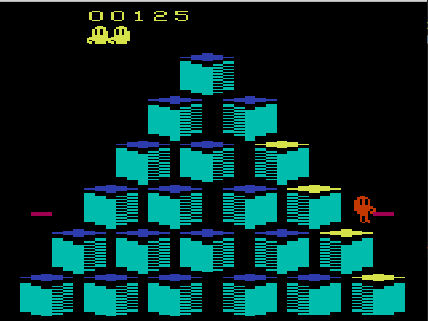
\includegraphics[width=\columnwidth]{screenshots/random_oscillations_2.png}
		\caption
		{Screen capture during Qbert's oscillation between two states.}
		\label{fig:random_oscillations}
	\end{figure}

	The weighted prior results can be seen in...
	
	% TODO: Tabulate score/level/screenshots for optimistic prior
	
	It was clear that using weighted prior led to much better results, since Qbert must visit all states in a level to complete it, and weighting the unvisited ones is intuitive.
	
	
	\section{Agent Performance} \label{sec:performance}
	% 30. as above, including analysis of effects of game events on agent behaviour and strategies (e.g., enemy avoidance) AND explanation of results over trials with multiple seeds to demonstrate generalization of learning
	
	To learn individual strategies, the \textsc{Subsumption} approach described by Mahadevan and Connell was employed \cite{mahadevan}. The agent is separated into three learners: \textsc{EnemyAvoider}, \textsc{FriendlyCatcher} and \textsc{BlockFinder}. The structure is shown in \cref{fig:subsumption}, where the ``S'' suppressor nodes denote priority, i.e., avoiding enemies takes priority over catching friendlies and going on blocks. This approach allows the agent to learn various aspects of the Qbert game independently, with a reduced state space for each task. This separation also makes intuitive sense, since learning how to avoid enemies should have little to do with finding blocks.
	
	\begin{figure}[!htb]
		\centering
		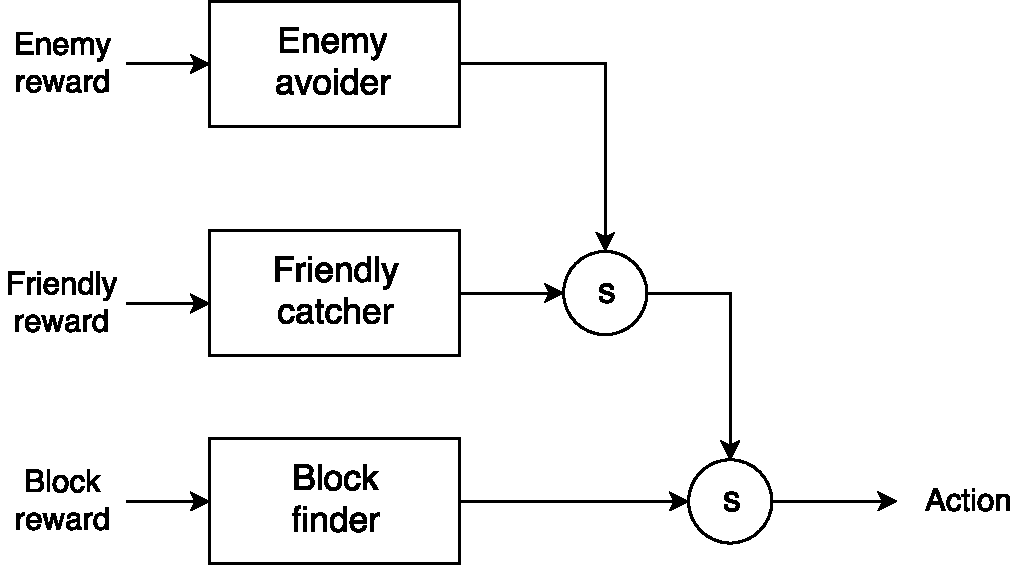
\includegraphics[width=\columnwidth]{plots/subsumption.pdf}
		\caption
		{Subsumption network used by the agent.}
		\label{fig:subsumption}
	\end{figure}

	\textsc{EnemyAvoider} is active whenever an enemy (``Coily'' and ``Purple Ball'') is close to Qbert, i.e. in any of the blocks directly adjacent to Qbert or 2 blocks away. An important strategy is to kill the purple snake enemy (``Coily'') by jumping on to the floating disks on the left and right of the board. If Coily is nearby, he will jump off the board, giving Qbert 500 points. This score is fed as a reward to the enemy avoider learner. As a penalty for dying to Coily, a negative reward of $-100$ is given to the learner. This combination of positive and negative reinforcement allows the agent to learn how to avoid and kill Coily.
	
	\textsc{FriendlyCatcher} is active whenever a friendly green agent (``Sam'' and ``Green Ball'') is within 2 blocks of Qbert. This learner encourages Qbert to catch Sam for 300 points and Green Ball for 100 points. Stopping Sam is also important because he changes the colors of blocks back to their original values, making Qbert do more work.
	
	\textsc{BlockFinder} is always active and keeps track of the colors of blocks within 2 blocks' distance of Qbert. It specifically keeps track of the number of adjacent blocks that are not of the desired color, encouraging Qbert to change them to their correct color to eventually complete the level.
	
	Note that, although one learner's decision always has priority for executing an action, multiple learners can still learn simultaneously. For example, while Qbert is avoiding an enemy, the block finder learner can still be learning from the actions being taken.
	
	% TODO: Show score as function of number of games played (with multiple seeds, game events [enemies])
	
	% TODO: Explain how game events were handled (with subsumption diagram and suppressor nodes, agents taking precedence over blocks...)
	
	\section*{Acknowledgments}
	
	There was a discussion with Andrei Purcarus and Andrew Lowther concerning the positions of various important bytes in the ALE RAM, including the bytes indicating a safe move update and the byte indicating a level change.
	
	
%	\renewcommand\refname{}
	\bibliographystyle{unsrt}
	\bibliography{readings}{}
	
\end{document}
